\chapter{Results}

This chapter will summarize the results achieved with the PTINY dialogue system.
We will describe the 2014 MTA App Quest admission in the first part.
Then we will go through the subjective user satisfaction results collected from CrowdFlower.
And finally we will compare the subjective user satisfaction between the Google and Kaldi ASR.

\section{App Quest 3.0}

At the beginning of February 2014, we participated in the contest App Quest 3.0\footnote{\url{http://2014mtaappquest.challengepost.com/}} by Metropolitan Transportation Authority (MTA)\footnote{\url{http://www.mta.info/}}.
The contest rules allowed teams and individuals around the globe and required to submit an application that utilizes at least one of the MTA data sets or APIs and includes the ability to update the data.

We registered at the Accessibility Innovation category because the primary features and functionality of PTINY best addresses end user with visual impairment.
Our keyword database can be actualized any time from the server and we utilize MTA data sets, therefore PTINY is eligible to participate.

The application was, however, required to run on one of many mobile or desktop platforms.
The PTINY is rather a phone service, therefore we decided to create a web page that enhance the accessibility even more.

A US number was provided by the department for the competition for which we employed three VMs.
We submitted PTINY\footnote{\url{http://challengepost.com/software/alex-information-about-public-transportation-in-new-york}} as an operational dialogue system, despite the fact that some features were not yet finished.

\subsubsection{PTINY web page}

The web page\footnote{\url{http://alex-ptien.com/}} created for the competition contains the overview of PTINY, examples of the features, terms of use and most importantly a ``try it now'' section shown in figure \ref{fig:mta}, in which a visitor can call PTINY directly through the web page.

\begin{figure}[ht]
\centering
\includegraphics[width=0.9\linewidth]{../img/mta.eps}
\caption{Web page with the \textit{"Call us Now"} button for the 2014 MTA App quest.}
\label{fig:mta}
\end{figure}

We utilized webrtc2sip gateway\footnote{\url{http://click2dial.org/u/index.html}} to create a \textit{Call us Now} button.
It allows any web browser with the support of WebRTC protocol to try out PTINY without the need of calling a number.
This includes mobile devices, too.

One additional VM was used for handling the button calls.

\subsubsection{PTINY demonstration video}

Another requirement was to provide a video link along with the submission.
The video should clearly explains the features and functionality through a comprehensive demonstration.
With the help of my colleague's voice, we created a video demonstrating the features by an example call with detailed description. \footnote{\url{https://youtu.be/wtlFCJj8faE}}
We also elevated the fact, that it can be a great asset for the visually impaired.

\subsubsection{Competition results}

Unfortunately we were not among the winners and there was no ranking either, so we do not know how close to winning we were.
Even more disappointing was the fact that we collected virtually zero calls.
As the rules state, judges are not required to test the application and may choose to judge based solely on the text description or demonstration video.
Our hope was that PTINY would attract at least curiosity of some other competitors.

However, the thing we cherish the most about our solution is that, while others are competing among each other within the same class of mobile applications, PTINY brings a new point of view on providing information about public transportation, with which a human can simply chat.


\section{CrowdFlower - subjective user satisfaction}

\todo{do výsledků říct kolik jobů jsme pustili a po jakých dávkách}




\subsection{Google ASR}

\begin{figure}[ht]
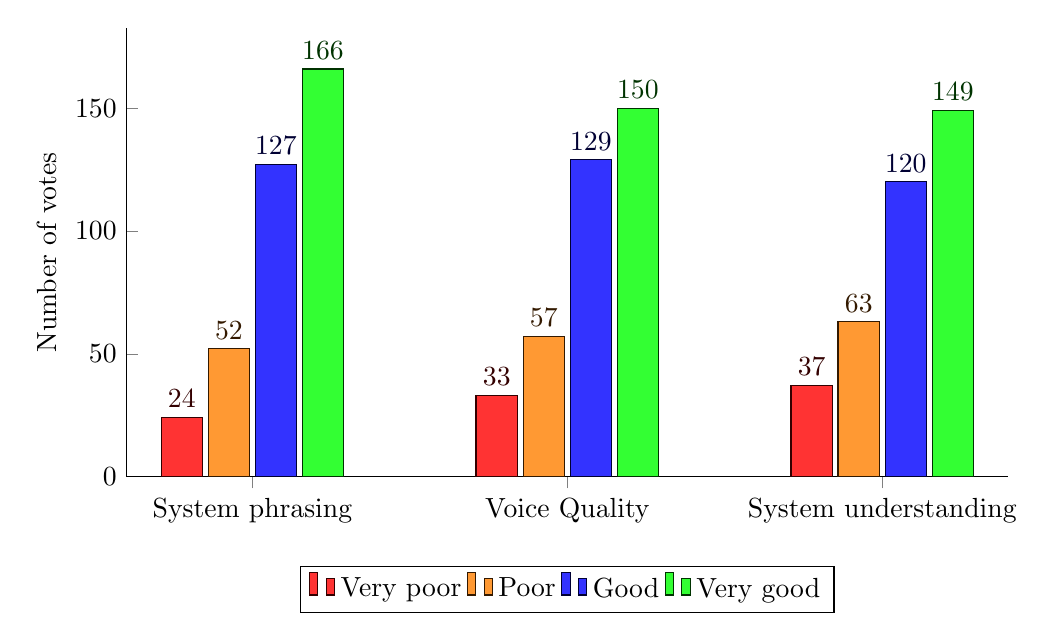
\begin{tikzpicture}
\begin{axis}[
    every axis plot post/.style={/pgf/number format/fixed},
    ybar,
    x=4cm,
    ymin=0,
    ylabel = Number of votes,
    %ymax=12,
    legend columns=-1,
	legend style={at={(0.5,-0.2)},anchor=north},
    xtick=data,
    enlarge x limits=0.2,
    bar width=15pt,
    symbolic x coords={1, 2, 3, 4},
    nodes near coords,
    axis lines*=left,
    xticklabels={System phrasing, Voice Quality, System understanding},
    xtick={1,...,3},
    ]

\addplot[red!20!black,fill=red!80!white] coordinates {(1,24) (2,33) (3,37)};
\addplot[orange!20!black,fill=orange!80!white] coordinates {(1,52) (2,57) (3,63)};
\addplot[blue!20!black,fill=blue!80!white] coordinates {(1,127) (2,129) (3,120)};
\addplot[green!20!black,fill=green!80!white] coordinates {(1,166) (2,150) (3,149)};
\legend{Very poor, Poor, Good, Very good}
\end{axis}
\end{tikzpicture}
\caption{Google histograms}
\label{fig:google}
\end{figure}

\subsection{Kaldi ASR}

\begin{figure}[ht]
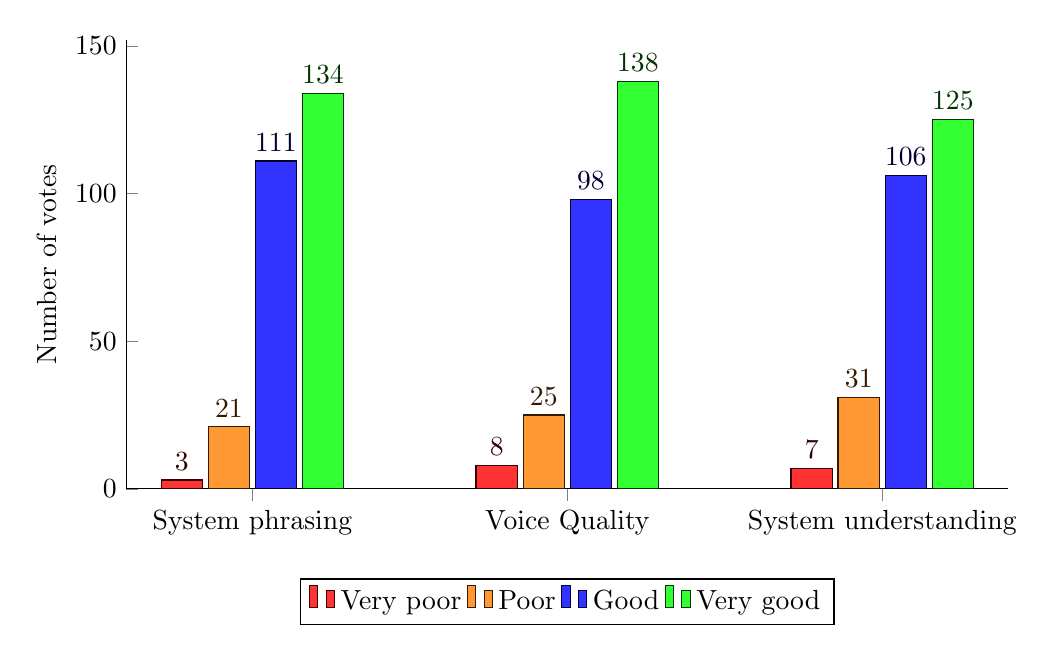
\begin{tikzpicture}
\begin{axis}[
    every axis plot post/.style={/pgf/number format/fixed},
    ybar,
    x=4cm,
    ymin=0,
    ylabel = Number of votes,
    %ymax=12,
    legend columns=-1,
	legend style={at={(0.5,-0.2)},anchor=north},
    xtick=data,
    enlarge x limits=0.2,
    bar width=15pt,
    symbolic x coords={1, 2, 3, 4},
    nodes near coords,
    axis lines*=left,
    xticklabels={System phrasing, Voice Quality, System understanding},
    xtick={1,...,3},
    ]

\addplot[red!20!black,fill=red!80!white] coordinates {(1,3) (2,8) (3,7)};
\addplot[orange!20!black,fill=orange!80!white] coordinates {(1,21) (2,25) (3,31)};
\addplot[blue!20!black,fill=blue!80!white] coordinates {(1,111) (2,98) (3,106)};
\addplot[green!20!black,fill=green!80!white] coordinates {(1,134) (2,138) (3,125)};
\legend{Very poor, Poor, Good, Very good}
\end{axis}
\end{tikzpicture}
\caption{Kaldi histograms}
\label{fig:kaldi}
\end{figure}


\begin{figure}[ht]
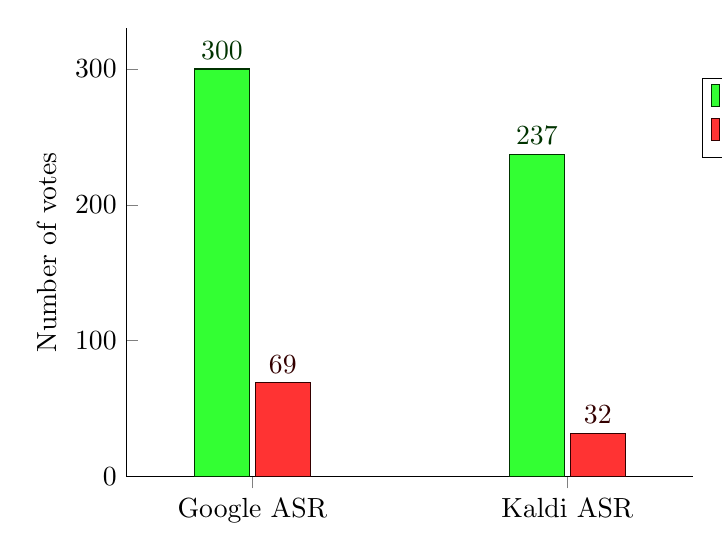
\begin{tikzpicture}
\begin{axis}[
    every axis plot post/.style={/pgf/number format/fixed},
    ybar,
    x=4cm,
    ymin=0,
    ylabel = Number of votes,
    %xlabel = Found what was looking for,
    %ymax=12,
    legend columns=1,
	legend style={
         overlay,
         at={(1.1,0.8)},
         anchor=center},
    xtick=data,
    enlarge x limits=0.4,
    bar width=20pt,
    symbolic x coords={1, 2},
    nodes near coords,
    axis lines*=left,
    xticklabels={Google ASR, Kaldi ASR},
    xtick={1,...,2},
    ]

\addplot[green!20!black,fill=green!80!white] coordinates {(1,300) (2,237)};
\addplot[red!20!black,fill=red!80!white] coordinates {(1,69) (2,32)};
\legend{Yes, No}
\end{axis}
\end{tikzpicture}
\caption{User satisfaction, have found what they were looking for}
\label{fig:us}
\end{figure}


\section{Future work}

\todo{to implement MTA API which would give us the ability to support more accurate information about current connections, locations of trains etc.}


\todo{implement MTA live data support which could be much more complexly used, to be able to ask how many minutes is the next train due our initial station would be cool}

% udělat, aby to rozumnělo na rohu páté a deváté -> vyinferovat street/avenue, nebo se i zeptat. Lidi ale nebyli v komunikaci tak familierní, aby používali takovýhle hantec, řikali to postupně a oficiálně, jakoby to zadávaly do vyhledávače. Což se zdá jen otázka času, kdy si lidi zvyknou a bude jim to přirozenější bavit se s počítačem jako se svým kámošem.


PTICS is focused on providing information relevant to prague integration transport. but we have to be more flexible than this. We wanted to support intersections as výchozí body, that is from fifth street and twenty second street or vice versa. We ended up supporting not only intersections but plain streets as valid input. This way one can go from fifth avenue even though it is not really an apt location.



\todo{Develop statistical SLU for robustness}


\section{Acknowledgements}

Access to computing and storage facilities owned by parties and projects contributing to the National Grid Infrastructure MetaCentrum, provided under the programme ``Projects of Large Infrastructure for Research, Development, and Innovations'' (LM2010005), is greatly appreciated.
%\pgfplotsset{ compat=1.9}

